\section{Grafer 2}
\subsection{Grafterminologi}

Der findes begreber til at beskrive kanter og knuder i ikke-orienterede grafer, som bl.a. beskriver hvordan knuder og kanter er orienterede i forhold til hinanden samt hvor mange knuder eller kanter, der er forbunde til en given knude.

\begin{defn}
To knuder $u$ og $v$ siges at være naboer i en ikke-orienteret graf $G$, hvis $u$ og $v$ er endepunkter i en kant $e$. Desuden siges kanten $e$ at forbinde $u$ og $v$, og $e$ er incident med både $u$ og $v$.
\end{defn}

\begin{defn}
En mængde af alle naboer til en knude $v$ i en graf $G=(V,E)$ betegnes $N(v)$ og kaldes et nabolag af $v$. Hvis $A$ er en delmængde af $V$, betegner $N(A)$ mængden af alle knuder i $G$, som er nabo til mindst én knude i $A$.
\end{defn}

\begin{defn}
Graden af en knude i en ikke-orienteret graf betegnes $deg(v)$ og er antallet af kanter incidente med den givne knude.  Et muligt loop vil bidrage med to grader til knuden. 
\end{defn}

En knude med grad 0 betegnes som værende \textit{isoleret} og har ingen incidente kanter. En knude med grad 1 betegnes som et \textit{vedhæng} og har netop én incident kant.

\begin{exmp}
Bestem graden af knuderne og nabolagene for knuderne i grafen i figur \ref{eksempel_nabo} og identificer isolerede knuder eller vedhæng.\\
Graden af en knude i grafen i figur \ref{eksempel_nabo} bestemmes ved at identificere antal incidente kanter til knuden. Derfor er $deg(A)=1$, $deg(B)=3$, $deg(C)=3$, $deg(D)=4$, $deg(E)=3$ og $deg(F)=2$. 
Nabolagene for de enkelte knuder er mængden af naboknuder. 
Derfor er $N(A)=\lbrace B \rbrace$, $N(B)=\lbrace A, C, D \rbrace$, $N(C)=\lbrace B, D, E \rbrace$, $N(D)=\lbrace B, C, E, F \rbrace$, $N(E)=\lbrace C, D, F \rbrace$ og $N(F)=\lbrace D, E \rbrace$. 
I grafen er A et vedhæng, og der forefindes ingen isolerede knuder.
\end{exmp}

\begin{figure}[h]
\centering
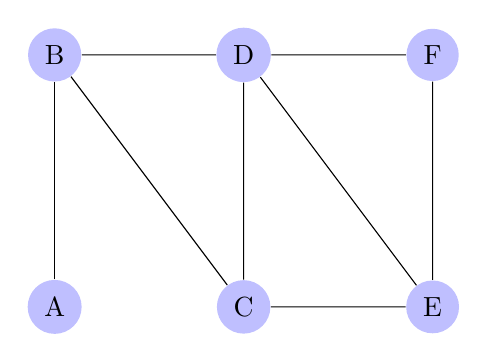
\begin{tikzpicture}
[scale=.8,auto=left,every node/.style={circle,fill=blue!25}]
  \node (n6) at (3,2) {A};
  \node (n4) at (3,6) {B};
  \node (n5) at (6,2) {C};
  \node (n1) at (6,6) {D};
  \node (n2) at (9,2) {E};
  \node (n3) at (9,6) {F};
  \foreach \from/\to in {n6/n4,n4/n5,n5/n1,n1/n2,n2/n5,n2/n3,n3/n1,n1/n4}
    \draw (\from) -- (\to);
\end{tikzpicture}
\caption{Simpel ikke-orienteret graf} \label{eksempel_nabo}
\end{figure}

For at beskrive summen af graderne for alle knuder i en graf anvendes \textit{The Handshaking Theorem}. 

\begin{thm}\label{handshake}
\textbf{The Handshaking Theorem}. Lad $G=(V,E)$ være en ikke-orienteret graf med $m$ kanter. Så er summen af knudernes grader \\
\begin{align*}
2m=\sum_{v \in V}deg(v)
\end{align*}
\end{thm}

\begin{proof}
I en ikke-orienteret graf med $m$ kanter, bidrager hver kant i en graf med to grader - én grad til hvert endepunkt. Det samlede antal grader for alle knuder i en graf stiger således med to pr. kant og summen af $deg(v)$ er $2m$. 
\end{proof}

Som følge af \ref{handshake} er summen af knudernes grader et lige tal. Derfor har en ikke-orienteret graf et lige antal knuder, hvor graden er et ulige tal.

\begin{thm}
En ikke-orienteret graf har et lige antal knuder af ulige grad. 
\end{thm}

\begin{proof}
Lad $V_1$ og $V_2$ være henholdsvis mængden af knuder af lige grad og mængden af knuder af ulige grad i en ikke-orienteret graf $G=(V,E)$ med $m$ kanter. Så er \\
\begin{align*}
2m=\sum_{v \in V}deg(v)=\sum_{v \in V_1}deg(v)+ \sum_{v \in V_2}deg(v)
\end{align*}
Da $deg(v)$ er lige for $v \in V_1$ er summen $\sum_{v \in V_1}deg(v)$ også lige. Summen af de to led på højresiden i ligningen er lige, fordi de tilsammen er lig $2m$, hvorfor $\sum_{v \in V_2}deg(v)$ også er lige. Summen $\sum_{v \in V_2}deg(v)$ består af en række ulige tal, og for at summen bliver lige, skal der således være et lige antal ulige led i summen.
Idet summen af graderne for knuderne af ulige grad i grafen er lige, må der være et lige antal af sådanne knuder.
\end{proof}




\subsection{Repræsentation af grafer}

Der er flere brugbare måder at repræsentere grafer på, og man ønsker i hvert tilfælde at vælge den pæneste repræsentation. \\
En overskuelig måde at repræsentere en graf på er ved matricer. To matricer, der almindeligvis bruges, er nabo-matricer, der er baseret på nabo-knuder, og incidens-matricer, baseret på incidensen af knuder og kanter. \\
Antag at $G=(V,E)$ er en simpel graf hvor $|V|=n$, hvor knuderne i $G$ står skrevet i vilkårlig rækkefølge som $v_1$, $v_2$, \dots , $v_n$. Nabo-matricen $A$ (eller $A_G$) af G er en $n \times n$ nul-et matrix, med 1 som den $(i,j)$’te indgang når $v_i$ og $v_j$ er naboer, og 0 er den $(i,j)$’te indgang, når de ikke er naboer. Hvis nabo-matricen er $A=[a_{ij}]$ så er

\begin{align*}
a_{ij}= \left\{\begin{array}{cc}
1 & hvis \  \lbrace v_i, v_j \rbrace \  er \  en \  kant \  i \  G \\
0 & ellers \\
\end{array}\right.
.
\end{align*}

En nabo-matrix af en graf er baseret på den valgte ordning af knuderne, hvorfor der kan være $n!$ forskellige nabo-matricer for en graf med $n$ knuder, i det der er $n!$ forskellige måder at ordne de $n$ knuder. Nabo-matricen for en simpel graf er symmetrisk, $a_{ij}=a_{ji}$, da begge indgange er 1, når de er naboer, og 0 ellers. Da en simpel graf ikke består af loops, er hver indgang $a_{ii},i=1,2,3, \dots ,n$ $0$. \\
Nabo-matricer kan også bruges til at repræsentere ikke-orienterede grafer med loops og flere kanter til samme knuder. Et loop ved en knude $v_i$ er repræsenteret ved 1 ved position $(i,i)$ i nabo-matricen. Når flere kanter forbinder det samme par af knuder $v_i$ og $v_j$, eller der er flere loops ved samme knude til stede, er nabo-matricen ikke længere en nul-et matrix, i det den $(i,j)$’te indgang af matricen er lig antallet af kanter forbundet til ${v_i,v_j}$. Alle ikke-orienterede grafer, herunder multi- og pseudografer, har symmetriske nabo-matricer. 

 \begin{equation*}
  \mathbf{A}=
  \begin{blockarray}{*{6}{c} l}
    \begin{block}{*{6}{>{$\footnotesize}c<{$}} l}
      A & B & C & D & E & F \\
    \end{block}
    \begin{block}{[*{6}{c}]>{$\footnotesize}l<{$}}
      0 & 1 & 0 & 0 & 0 & 0 \bigstrut[t]& A \\
      1 & 0 & 1 & 1 & 0 & 0 \bigstrut[t]&B \\
      0 & 1 & 0 & 1 & 1 & 0 \bigstrut[t]&C \\
      0 & 1 & 0 & 1 & 1 & 0 \bigstrut[t]& D \\
      0 & 0 & 1 & 1 & 0 & 1 \bigstrut[t]& E \\
      0 & 0 & 0 & 1 & 1 & 0 \bigstrut[t]& F \\
    \end{block}
  \end{blockarray}
\end{equation*}

En anden almindelig måde at repræsentere grafer på er ved incidens-matricer. Lad $G=(V,E)$ være en ikke-orienteret graf. Antag at $v_1$, $v_2$, \dots , $v_n$ er knuder og $e_1$, $e_2$, \dots , $e_n$ er kanter i G. Incidens-matricen, i forhold til ordningen af $V$ og $E$, er en $n x m$ matrix $M=[m_{ij}]$, hvor 
\begin{align*}
m_{ij}= \left\{\begin{array}{cc}
1 & hvis \  {e_j} \  er \  nabo \ til \ v_i \\
0 & ellers \\
\end{array}\right.
\end{align*}

Incidens-matricer kan også bruges til at repræsentere flere kanter og loops. Flere kanter ved én knude er repræsenteret i incidens-matricen ved kolonner med identiske indgange, i det disse kanter er incidente med det samme par af knuder. Loops er repræsenteret ved en kolonne med præcis én indgang lig 1, der svarer til den knude, der er incident med loopet. 

 \begin{equation*}
  \mathbf{M}=
  \begin{blockarray}{*{8}{c} l}
    \begin{block}{*{8}{>{$\footnotesize}c<{$}} l}
      1 & 2 & 3 & 4 & 5 & 6 & 7 & 8 \\
    \end{block}
    \begin{block}{[*{8}{c}]>{$\footnotesize}l<{$}}
      1 & 0 & 0 & 0 & 0 & 0 & 0 & 0 \bigstrut[t]& A \\
      1 & 1 & 1 & 0 & 0 & 0 & 0 & 0 \bigstrut[t]&B \\
      0 & 1 & 0 & 1 & 1 & 0 & 0 & 0 \bigstrut[t]&C \\
     0 & 0 & 1 & 1 & 0 & 1 & 1 & 0 \bigstrut[t]& D \\
      0 & 0 & 0 & 0 & 1 & 1 & 0 & 1 \bigstrut[t]& E \\
     0 & 0 & 0 & 0 & 0 & 0 & 1 & 1 \bigstrut[t]& F \\
    \end{block}
  \end{blockarray}
\end{equation*}


\usetikzlibrary{arrows, positioning}
\begin{figure}[!h]
  \centering
  \begin{tikzpicture}[shorten >=1pt,node distance=3cm,on grid,auto]
    \tikzstyle{state}=[shape=circle,thick,draw,minimum size=1.5cm]

    \node[state] (A1) {$B$};
    \node[state,above of=A1] (B1) {$D$};
    \node[state,above of=B1] (C1) {$F$};

    \node[state,right of=A1] (A2) {$A$};
    \node[state,above of=A2] (B2) {$C$};
    \node[state,above of=B2] (C2) {$E$};



    \path[-,draw,thick]
    (A1) edge node {$e_1$} (A2)
    (A1) edge node {$e_3$} (B1)
    (A1) edge node {$e_2$} (B2)
    (B1) edge node {$e_4$} (B2)
    (B1) edge node {$e_7$} (C1)
    (C1) edge node {$e_8$} (C2)
    (C2) edge node {$e_5$} (B2)
    (C2) edge node {$e_6$} (B1)

    ;

  \end{tikzpicture}
  \caption{Model}
  \label{fig:f1}
\end{figure}




